%Standard imports für Artikel
\documentclass[12pt]{article}
\usepackage[utf8]{inputenc}
\usepackage[ngerman]{babel}
\usepackage[T1]{fontenc}
\usepackage{cite}
\usepackage{todonotes}

%Bilder importieren
\usepackage{graphicx}
\graphicspath{ {./img/} }

\usepackage{hyperref}
\hypersetup{
    colorlinks,
    citecolor=black,
    filecolor=black,
    linkcolor=black,
    urlcolor=black
}

\setlength{\parskip}{1em}

\title{Human Centered Design - Software zur Terminvereinbarung}
\author{Johannes Schnirring}

\begin{document}

\begin{titlepage}
    \centering
    {\scshape\LARGE Human Centered Design - Software zur Terminvereinbarung \par}
    \vspace{1cm}

    {\scshape\Large Bachelorarbeit\par}
    \vspace{1.5cm}

    \begin{tabular}{r l}
        {\Large Studierender:} & {\Large Johannes Schnirring}             \\ \\
        {\Large Betreuung:}    & {\Large Prof. Dr. Claude Draude        } \\ \\
        {\Large Semester:}     & {\Large Wintersemester 2022}             \\ \\
        {\Large Datum:}        & {\Large \today}                          \\ \\
    \end{tabular}
    \vfill
    {\large Universität Kassel}

    % Bottom of the page

\end{titlepage}

%\maketitle
\tableofcontents
\newpage

\section{Einleitung}

\subsection{Motivation}

% Hier wird die Problemstellung im Kontext
% einer Anwendung dargestellt und der Inhalt der Arbeit kurz vorweggenommen. Welches Problem wurde
% gelöst, warum ist das relevant? Wie ist die Vorgehensweise? Was wurde thematisch eingegrenzt, was
% wurde ausgegrenzt? Wichtig ist es, den eigenen Beitrag in wenigen prägnanten Sätzen herauszuarbeiten. (Das Fazit soll sich zum Schluss auf diese Beiträge beziehen, um der Arbeit eine erzählerische
% Klammer zu geben.) Die Einleitung endet mit einem Überblick über die Arbeit – hierbei werden die
% Inhalte der einzelnen Kapitel knapp umschrieben

Der Ansatz des Human Centered Design bietet einen nutzungsfokussierten
Blickwinkel auf den Entwurf und den Designprozess von Software. In dieser
Ausarbeitung werden die grundlegenden Methoden des Human Centered Design
vorgestellt, praktisch angewendet und abschließend reflektiert.

Die allgemeine Studienberatung und Information Studium der Universität Kassel
nutzt zur Erleichterung und Dokumentation der täglich anfallenden Aufgaben eine
speziell für diesen Bereich entwickelte, webbasierte Software. Diese Software
setzt sich aus verschiedenen Modulen zusammen, die dazu beitragen Ordnung und
Kommunikation im Team zu erleichtern. Um allen Mitarbeitenden einen Überblick
zu geben, welche Kolleg:innen aufgrund von Urlaub, Krankheit oder Dienstreisen
am aktuellen Tag abwesend sind, gibt es in dieser Software ein Modul um
Abwesenheiten einzupflegen und somit alle Teammitglieder auf dem neuesten Stand
zu halten.\\ Um die Nutzung des Abwesenheitsmoduls für alle Mitarbeitenden der
Abteilung intuitiver und einfacher zu gestalten soll eine Überarbeitung des
Moduls mit Methoden des Human Centered Design durchgeführt werden. Ziel ist die
Implementierung eines übersichtlichen und intuitiven Managements von
Abwesenheiten des Teams in der bestehenden Callcenter Software.

Das Ziel dieser Seminararbeit ist es den Designprozess strukturiert zu
begleiten und zu dokumentieren. Am Beispiel des Abwesenheitsmoduls sollen
Verfahren zur Entwicklung und Einführung intuitiv zu bedienender Software in
enger Zusammenarbeit mit den Anwender:innen diskutiert und praktisch erprobt
werden. Hierfür wird zunächst der Begriff des Human Centered Design näher
erläutert. Mit dem \textit{Interview im Kontext} wird eine grundlegende Methode
dieses Designansatzes vorgestellt. Der Ablauf des Interviews in der Praxis wird
im Hauptteil beschrieben. Die darauf aufbauenden Prozesse der Erarbeitung von
Optimierungen der Software werden weitergehend dokumentiert. Schließlich werden
die ersten Entwürfe der neu umgesetzten Veränderungen präsentiert und kritisch
reflektiert. Abschließend wird der Erfolg der verwendeten Methoden beurteilt
und ein Ausblick auf die weiteren Schritte der Implementierung gegeben.

\section{Methoden}

\subsection{Human Centered Design}
Human-Centered Design ist eine Methode zur Entwicklung interaktiver Systeme,
wie beispielsweise Software. Der wichtigste Aspekt der Methode ist es, diese
Systeme benutzerfreundlich und möglichst nützlich zu gestalten. Wie Alan Dix
klarstellt hat sich die Interaktion zwischen Menschen und Computern in den
letzten Jahrzehnten stark verändert. Während Computer anfangs die meiste Zeit
einfach vor sich hin gerechnet haben, sind Softwaresysteme heutzutage höchst
interaktiv uns sollen ohne Hürden von allen Teilen der Gesellschaft genutzt
werden können. \cite{hci}[S. 234] Beim Human Centered Design werden die
Nutzenden der Systeme in den Mittelpunkt gestellt. Martin Ludwig Hofmann
betont: \glqq [Es geht nicht darum] vom Gerät her zu denken, sondern vom
Menschen und der Art und Weise, wie er die Welt wahrnimmt\grqq{}. \cite{hcd}[S.
    134] Die Bedürfnisse, Prozessabläufe und Erwartungen der Nutzenden sind beim
Human Centered Design der wichtigste Aspekt beim Entwurf von Schnittstellen
zwischen Systemen und den Menschen, die sie benutzen.

Die Nutzenden sollen während der gesamten Design- und Entwicklungsphase
kontinuierlich in den Prozess der Produktentwicklung eingebunden werden. Statt
sie eine fertige Idee oder einen fertig entwickelten Prototypen bewerten zu
lassen, sollen ihre Bedürfnisse erforscht und direkt in die Ausgestaltung des
Produkts integriert werden. In \textit{Human-Computer Interaction} wird betont
wie wichtig es ist den Fokus im gesamten Prozess auf die Nutzenden zu legen.
Bei allen Aspekten des Softwaredesigns ist es wichtig, das direkte Feedback der
Nutzenden einzuholen und in den kompletten Entwicklungs- und Lebenszyklus einer
Software einfließen zu lassen \cite{hci}[S. 226]

Der Designprozess beinhaltet den intensiven Austausch mit den Nutzenden. In
\textit{The human-computer interaction handbook} weisen die Autoren auf die
Relevanz von Beobachtung und aufmerksamer Wahrnehmung hin. Wenn man Nutzende
fragt, wie sie eine Software benutzen, werden sie viele Dinge nicht erwähnen,
weil sie vergessen werden, nicht relevant erscheinen oder die Nutzenden nicht
genau wissen, wie sie darüber sprechen können. \cite{hciHandbook}[S. 970]
Resultierend ist es also wichtig die Bedürfnisse, Fähigkeiten und Strategien
der Nutzenden direkt im Nutzungsalltag zu beobachten und zu analysieren.
Entwickler und Designer sollen aber auch das Umfeld, die Arbeitsabläufe und den
Kontext des zu entwerfenden Systems genau verstehen. So soll ein System
entwickelt werden, dass den Nutzenden in ihrer Situation genau den Mehrwert
bieten kann, der für sie wichtig ist. Das System soll sich an die Abläufe und
Prozesse der Nutzenden anpassen und nicht umgekehrt.

\begin{figure}[h]
    \caption{Iteratives Vorgehen im Human Centered Design nach ISO 9241 \cite{iso9241}}
    \centering
    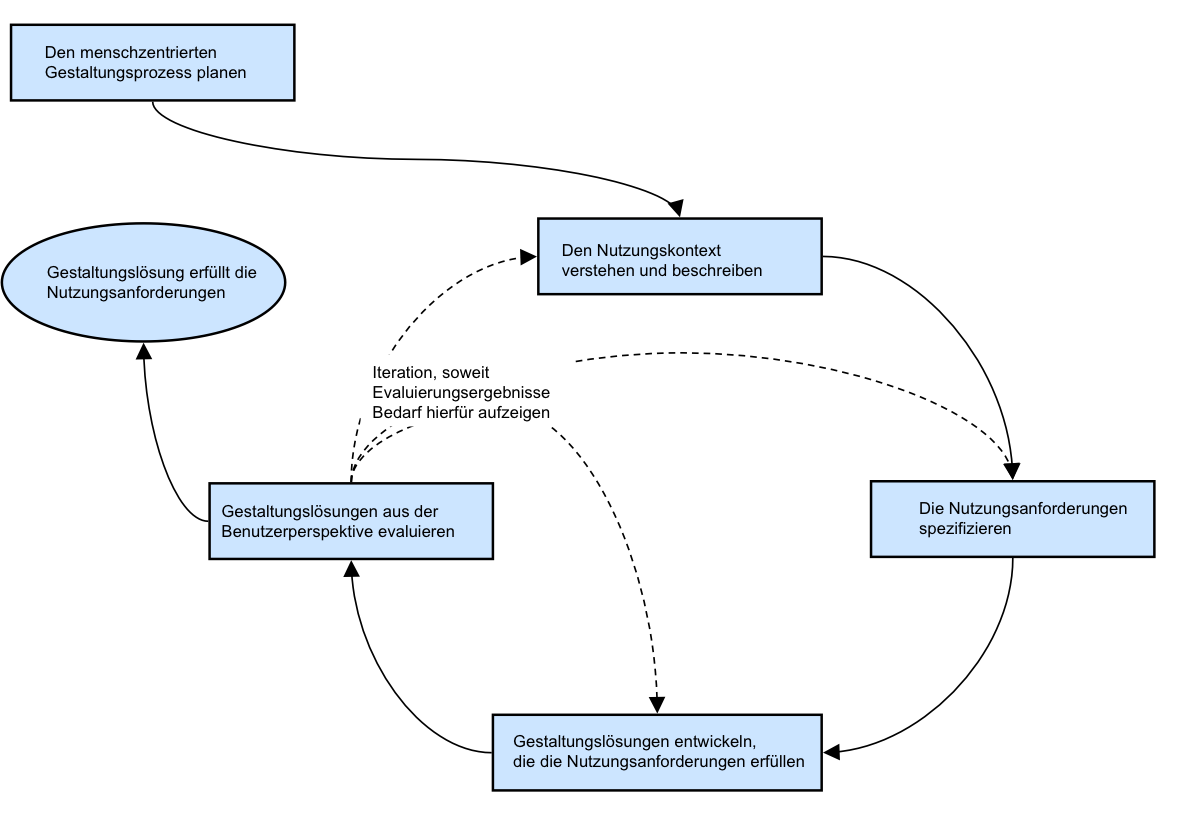
\includegraphics[width=10cm]{HCD.png}
\end{figure}

Alan Dix stellt des weiteren ganz klar heraus, dass dieser Prozess in mehreren
Iterationen ablaufen muss. Nach dem ausgiebigen Beobachten und Diskutieren der
Anforderungen gemeinsam mit den Nutzenden, können erste Prototypen und
Beta-Versionen entwickelt werden. Diese müssen nun unbedingt erneut mit den
Nutzenden ausprobiert und diskutiert werden. Dieser Prozess des Ausprobierens,
Beobachtens, Analysierens und Entwickelns neuer Lösungsansätze sowie deren
praktische Umsetzung muss oftmals in vielen Iterationen wiederholt und mit
jedem Mal weiter optimiert werden.\cite{hci}[S. 234-237]

\subsection{Interview im Kontext}
Eines der wichtigsten Kernkonzepte im Human Centered Design ist das Verstehen
der Nutzenden und ihrer Umfelder. Hierfür gibt es verschiedene Methoden, die
Entwicklern und Designern diesen Prozess erleichtern. An dieser Stelle wird die
Methode des\textbf{ Interviews im Kontext} gewählt und kurz vorgestellt.

Ziel des \textit{Interviews im Kontext} ist es, die Anforderungen und
Bedürfnisse der Nutzenden im realen Nutzungskontext zu erleben und zu
dokumentieren. Wie in \textit{Contextual Design} klargestellt wird, machen
klassische Techniken der Marktforschung für eine nutzerfokussierte
Softwareentwicklung oftmals keinen Sinn. Wichtig ist es die Nutzenden im
tatsächlichen Arbeitsumfeld zu beobachten und somit den Kontext der Interaktion
mit der Software als essentiellen Teil in die Beobachtungen einfließen zu
lassen.\cite{contextualDesign}[S. 36ff] Hierbei werden die Nutzenden direkt an
Ihrem Arbeitsplatz, während ihrer Arbeit beobachtet und begleitet. Der
Interviewende begibt sich hauptsächlich in eine zurückhaltende Rolle eines
Beobachters. Wie in \textit{The human-computer interaction handbook}
vorgeschlagen, wird der Rahmen des Interviews möglichst locker gehalten. Die
Nutzenden des Systems sollen möglichst natürlich und frei zeigen, wie sie das
System benutzen.\cite{hciHandbook}[S. 972] Wichtig ist den Nutzenden
Möglichkeiten zum Erzählen zu bieten. Auch Dinge die im ersten Moment trivial
oder nicht relevant erscheinen, sollen Nutzende in Ruhe ausführen und dem
Interviewer somit die Möglichkeit geben, einen umfassenden Einblick in die
Interaktionen mit dem System zu gewähren. Der Interviewende verbringt also die
meiste Zeit damit zuzuhören und Impulsen des Interviewten zu folgen. Zusätzlich
stellt er Nachfragen zum besseren Verständnis der beobachteten Situationen,
Arbeitsabläufe und Handlungen. Der Interviewende hält das Feedback der
Nutzenden zusammen mit seinen eigenen Beobachtungen meist schriftlich fest.
Ziel dieser Methode ist es kontextabhängige Nutzungsszenarien der Systeme
mitzuerleben, zu dokumentieren und daraus Ideen für die Entwicklung bzw.
Verbesserung der Systeme zu gewinnen.

\subsection{Weitere Methode (vllt Prototypentwicklung/Feedbackmethode)}

\section{Durchführung}

Struktur abarbeiten und verschiedene inhaltliche Aspekte immer wieder
aufgreifen. Oder inhaltliche Aspekte abarbeiten und Struktur
aufgreifen...?\todo{Struktur?}

\subsection{Situation in der Abteilung}

\paragraph{Überleitung Situation Abteilung}
Um den Bedarf und Entstehungsprozess der Software besser einordnen zu können,
werden nun die Workflows und Prozessabläufe im Büroteam kurz skizziert. Die
Beschreibung der Situation im Team hilft zu erkennen, wie sich die aktuelle
Softwarelösung in den Arbeitsalltag eingliedert, welche Prozessabläufe bereits
gut durch Software begleitet werden, und an welchen Stellen noch
Optimierungsbedarf besteht.

\paragraph{Grundlegende Beschreibung der Abteilung}
Als Nutzergruppe aller Studien dieser Bachelorarbeit werden die Mitarbeitenden
einer Abteilung der Hochschulverwaltung an der Universität Kassel dienen. Es
handelt sich um die Abteilung "Studium und Lehre", zu deren alltäglichen
Aufgaben es gehört, alle erdenklichen Organisationen zu übernehmen, die
Studierenden und Lehrenden ein erfolgreiches Zusammenarbeiten an der
Universität ermöglichen. Hierzu gehören beispielsweise das Einschreiben, und
Exmatrikulieren von Studierenden, die Durchführung des Bewerbungsverfahrens,
das Betrieben der Information Studium und die allgemeine Studienberatung. In
dieser Arbeit wird der Fokus auf die Mitarbeitenden der Studienberatung in der
Abteilung Studium und Lehre gesetzt.

\paragraph{Studienberatung}
Die allgemeine Studienberatung der Universität Kassel berät Studierende zu
allen Fragen rund um das Studium. Insbesondere bei persönlichen Problemen mit
der Fertigstellung des eigenen Studiums hilft die Studienberatung mit einem
persönlichen Lösungsgespräch und kann an weitere fachspezifische
Beratungsstellen weiter vermitteln. Des Weiteren bietet die allgemeine
Studienberatung verschiedene Workshops und Seminare an. Hierbei können sich
Studierende in Gruppen mit Fokus auf bestimmten Fragestellungen austauschen und
Qualifikationen im Umgang mit herausfordernden Studiensituationen erlangen.
Auch "Schnupperkurse" für Studieninteressierte und Schüler werden von der
allgemeinen Studienberatung angeboten um jungen Menschen mit Interesse an einem
Studium einen möglichst unmittelbaren Einblick in den Studienalltag zu
gewähren.\cite{studBeratungKsWeb}

\paragraph{Terminvereinbarung in der ZSB}
Eines der zentralen Themen im Alltag der Studienberatung sind Beratungstermine.
\todo{gendern?} Studienberatende müssen Termine mit den Ratsuchenden
vereinbaren und abstimmen. Beratungstermine können über verschiedene
Kontaktkanäle stattfinden: Es ist eine telefonische Beratung oder auch eine
Beratung über eine Videokonferenz möglich. Selbstverständlich ist auch möglich
einen persönlichen Beratungskontakt vor Ort zu vereinbaren. Über all diese
Termine muss jeder Studienberatende den Überblick behalten und gleichzeitig
neue Terminanfragen schnell beantworten können. Um diesen Prozess zu
erleichtern und mögliche Fehler, wie beispielsweise Terminüberschneidungen, zu
minimieren, wird hierfür die \textbf{Software "Stubegru"} eingesetzt.

\subsection{Aktuelle Softwarelösung}
\paragraph{Stubegru}
Stubegru ist ein umfangreiches Softwarepaket für akademische Beratungsstellen.
Die webbasierte Groupware begleitet viele Arbeitsabläufe im Alltag einer
Beratungsstelle an einer Hochschule. In einem Softwaresystem vereint Stubegru
eine Wissensdatenbank in Form eines Wikis, sowie ein Dashboard mit vielen
Modulen für spezifische Workflows. So können über Stubegru an der Universität
Kassel beispielsweise Abwesenheiten der Abteilung, Telefonnotizen und
Beratungskontakte verwaltet werden. Jeder Mitarbeitende der Abteilung hat über
einen eigenen Account Zugriff auf die Software, die er im Browser aufrufen
kann. Die Software hilft dabei tagesaktuelle Informationen schnell und
übersichtlich allen Mitarbeitenden zur Verfügung zu stellen und bei Bedarf
langfristige und ausführliche Informationen mit wenigen Klicks zur Verfügung zu
stellen.\cite{stubegruWebsite}

\paragraph{Terminvereinbarung in Stubegru}
Das wichtigste Modul der eingesetzten Software für die Studienberatung ist der
Kalender zur Terminvereinbarung von Beratungsterminen. Über diese Modul können
in einem zweistufigen Prozess Termine für Ratsuchende freigegeben und an die
entsprechenden Studierenden und Studieninteressierten vermittelt werden.

\paragraph{Zeitslots erstellen}
Im ersten Schritt können die Studienberatenden freie Zeitslots für ihre
Beratungstermine anlegen. Diese Zeitslots zeigen an, dass der entsprechende
Beratende in der eingestellten Zeitspanne potenziell Zeit für ein
Beratungsgespräch hat. Bei der Erstellung der Zeitslot können weitere Attribute
wie der Beratungskanal (Online Meeting, Telefongespräch oder Präsenztermin)
konfiguriert werden. Außerdem können Mail Templates verknüpft werden, die im
Falle einer Terminvergabe den Ratsuchenden per Email über alle wichtigen
Informationen zum Termin informieren.

\paragraph{Terminvergabe durch Erstinformation}
Im zweiten Schritt werden die eingestellten Zeitslots durch Hilfskräfte der
Erstinformation an Ratsuchende vergeben. Die Erstinformation der Universität
Kassel berät Studierende und Studieninteressierte zu allen Fragen rund ums
Studium übers Telefon, Email und eine Servicetheke vor Ort. Bei tiefgehenden
Fragen und spezifischen Anliegen verweisen die Mitarbeitenden an die
entsprechenden Sachbearbeitenden oder Beratungsstellen. Die Erstinformation ist
auch für das vereinbaren von Beratungsterminen mit der allgemeinen
Studienberatung verantwortlich. Sind die Mitarbeitenden der Erstinformation in
Kontakt mit einem Kunden, der einen Termin in Anspruch nehmen möchte, können
sie in der Software alle freien Zeitslots der Beratenden einsehen und einen
passenden Termin mit den Kunden vereinbaren. Wenn ein freier Zeitslot vergeben
wird und fest mit einem Ratsuchenden verknüpft ist, wird eine Email an den
Beratenden versendet, der über alle Details wie Adresse, Kontaktinformationen
und Anliegen der Ratsuchenden informiert wird. Des Weiteren wird eine Mail an
die Ratsuchende Person versendet, die auf dem zuvor verknüpften Mailtemplate
aufbaut und dynamisch terminrelevante Informationen einsetzt, wie
beispielsweise Datum und Zeit des Termins, oder eine Wegbeschreibung zum
Beratungsraum.

\paragraph{Auskunft bei Terminabsage}
Eine weitere Verwendung des Kalendermoduls tritt ein, wenn Kunden der
Erstinformationen Fragen zu einem bereits vereinbarten Termin haben oder diesen
Absagen möchten. In diesem Fall können die Hilfskräfte der Erstinformation über
eine Suchfunktion gezielt nach den vereinbarten Terminen des Kunden suchen und
weitere Auskünfte geben.

\paragraph{Datenschutz}
Da Datenschutz in Beratungsszenarien eine wichtige Rolle einnimmt, kann
lediglich der verantwortliche Beratende das Anliegen der ratsuchenden Person
einsehen. Zu Auskunftszwecken können aber alle Mitarbeitenden der Abteilung
sehen, wann ein Beratungstermin mit welchem Beratenden vereinbart wurde.
Datensätze zu vergangenen Beratungstermin werden täglich gelöscht, sodass
möglichst wenig personenbezogenen Daten in der Datenbank gespeichert werden
müssen. Über ein differenziertes Berechtigungssystem der eingesetzten Software
Stubegru, kann genau gesteuert werden, welche Nutzergruppen Beratungstermine
anlegen und vergeben dürfen.

\subsection{Grund für Veränderung}

\paragraph{Neue Softwareversion}
Die Software Stubegru wurde ursprünglich von einer Hilfskraft der Abteilung
Studium und Lehre an der Universität Kassel erstellt und betreut. Da die
Software nun langfristig an der Uni Kassel und auch an anderen deutschen
Hochschulen eingesetzt werden soll, wurde ein Prozess gestartet, um eine
Professionalisierung und nachhaltige Betreuung der Software zu gewährleisten.
In diesem Rahmen wurde die Software auch für andere Hochschulen zur Verfügung
gestellt und unter einer OpenSource Lizenz veröffentlicht. Im Zuge dieser
Veröffentlichung wurde in Zusammenarbeit mit der Hochschule Bremen eine
grundlegend überarbeitete Variante der Software Stubegru erstellt, die im
Vergleich zu der bisherigen Version deutlich flexibler ist und mehr
Anpassungsmöglichkeiten bietet. Wie Erich Gamma in \textit{Elemente
    wiederverwendbarer objektorientierter Software} betont, bieten wiederverwendbar
gestaltete Softwarestrukturen und abstrakte Implementierungsansätze die Option,
Softwaremodule in verschiedenen Kontexten zu verwenden. Dies erfordert im
Softwareentwurf allerdings eine vorausschauende Planung und einen hohen
Abstraktionsgrad.\cite{wiederverwSoftware} Somit ist der Einsatz der Software
Stubegru an verschiedenen Hochschulen mit verschiedenen Arbeitsabläufen
realisierbar. Um von dieser neuen, überarbeiteten Softwareversion auch an der
Universität Kassel zu profitieren, ist wiederrum eine grundlegende
Überarbeitung des Moduls zur Terminvergabe der Beratungstermine für die
allgemeinen Studienberatung notwendig.

\paragraph{Fehlende Features}
In der aktuellen Softwareversion gibt es einige Features, die noch nicht
vollständig funktionieren oder nicht optimal auf den tatsächlichen
Arbeitsalltag zugeschnitten sind. An diesen Stellen soll das neue Modul zur
Terminvereinbarung verbessert und noch weiter an die Bedürfnisse der Nutzenden
angepasst werden. Im Rahmen der Softwareüberarbeitung mit der Hochschule Bremen
wurde für die neue Version von Stubegru bereits ein Kalendermodul zur Vergabe
von Beratungsterminen entwickelt. Dieses Modul weist allerdings noch einige
Probleme auf, um reibungslos im Arbeitsalltag der allgemeinen Studienberatung
an der Universität Kassel eingesetzt zu werden. In der "Bremer Version" läuft
das Erstellen und Vergeben eines Beratungstermins in einem einzigen Schritt ab.
Ein zentraler Punkt um die überarbeitete Software auch in der allgemeinen
Studienberatung der Universität Kassel nutzen zu können ist der zweistufige
Prozess der Terminvergabe. Hier müssen Beratende die Möglichkeit haben zuerst
freie Terminslots freizugeben, die dann in einem getrennten zweiten Schritt
durch Mitarbeitende der Erstinformation an Ratsuchende vergeben werden können.

\paragraph{Vorschau auf Hauptteil der Arbeit}
Welche Anpassungen im Detail notwendig sind, um die Software optimal in der
Studienberatung einsetzen zu können, soll in den folgenden Kapiteln methodisch
herausgearbeitet werden und durch Dokumentation von praktische durchgeführten
Nutzerstudien und Gesprächen mit den verantwortlichen Personen ergänzt werden.
Diese Bachelorarbeit soll insbesondere den Designprozess strukturiert begleiten
und wissenschaftliche Methoden aufzeigen, um Softwareentwicklern und Nutzenden
eine möglichst gute Zusammenarbeit zu ermöglichen.

\subsection{Erste Planungen - Interview im Kontext}

\paragraph{Warum Interview im Kontext?}
Das Modul zur Terminvereinbarung der Software Stubegru soll auf den
Arbeitsalltag der allgemeinen Studienberatung der Universität Kassel angepasst
werden. Dies soll mit Methoden des Human Centered Design umgesetzt werden. Ein
zentraler Bestandteil des Human Centered Design ist der enge und stetige
Austausch mit den Nutzenden des Softwaresystems \cite{hci} \todo{Quelle
    checken} Um den Änderungsbedarf eines bestehenden Softwaresystems einschätzen
zu können wird im Human Centered Design häufig die Methode des
\textit{Interviews im Kontext} gewählt.\cite{contextualDesign} Diese Methode
eignet sich besonders zu Beginn des Entwicklungsprozesses, da wenig
Vorkenntnisse über die eingesetzte Software und das Umfeld, in dem Software
eingesetzt wird, bekannt sein muss. Die Softwareentwickler können so einen
guten Einstieg finden, um einen Überblick zu gewinnen, welche Funktionen die
fertige Software am Ende unterstützen muss. Auch lässt sich durch ein genaues
Beobachten beim Interview herausarbeiten, in welchem Kontext die Software im
tatsächlichen Arbeitsalltag genutzt wird und welche weiteren Faktoren die
Nutzenden der Systeme beeinflussen.

\subsubsection{Kontext des Interviews}

\paragraph{Rahmenbedingungen IiK}
Als erster Schritt wurde ein Termin für ein Interview im Kontext mit Oliver
Claves \todo{Namen nennen?} vereinbart. Herr Claves ist einer von drei
Mitarbeitenden der allgemeinen Studienberatung der Universität Kassel. Zu
seinen Aufgaben gehört die Betreuung der Software Stubegru und deren Einsatz in
der Abteilung Studium und Lehre. Seit über sechs Jahren arbeitet Oliver Claves
bereits gemeinsam mit Hilfskräften an dem Aufbau und der Optimierung der
Software Stubegru um den täglichen Arbeitsalltag seines Teams optimal zu
unterstützen. \todo{Ich-Perspektive?} Ich habe mich persönlich mit Oliver
Claves in seinem Büro im Campus Center der Universität getroffen. Dort hat er
mir an seinem Schreibtisch gezeigt, wie er mit der alten Version der Software
Beratungstermine erstellt und vergeben kann. Herr Claves saß vor mir und hatte
Maus und Tastatur in der Hand. Ich saß hinter ihm auf einem Stuhl und habe auf
einem iPad Notizen mitgeschrieben. Für die Dauer von einer Stunde hat Herr
Claves mir gezeigt, wie er die Software aktuelle nutzt, welche Features für ihn
sehr wichtig sind und an welchen Stellen noch Verbesserungspotenzial besteht.

\paragraph{Detaillierter Ablauf IiK}
Am Anfang habe ich Herr Claves gebeten, mir einmal zu zeigen, wie er einen
Beratungstermin in der Software anlegen und vergeben kann. Dies ist der
Workflow, der im Arbeitsalltag am häufigsten vorkommt und daher eine hohe
Priorität im Designprozess hat. Herr Claves klickte sich durch die
verschiedenen Eingabefelder um einen freien Zeitslot für einen Beratungstermin
anzulegen. Hierbei erwähnte er, dass es ganz wichtig ist, dass Datum und
Uhrzeit des Beratungstermins mit wenigen Klicks über ein Date-/Timepicker mit
der Maus eingeben werden können. Eine Datumseingabe über die Tastatur würde er
nicht bevorzugen.

\begin{figure}[h]
    \caption{Datepicker im Formular zur Erstellung eines Zeitslots}
    \centering
    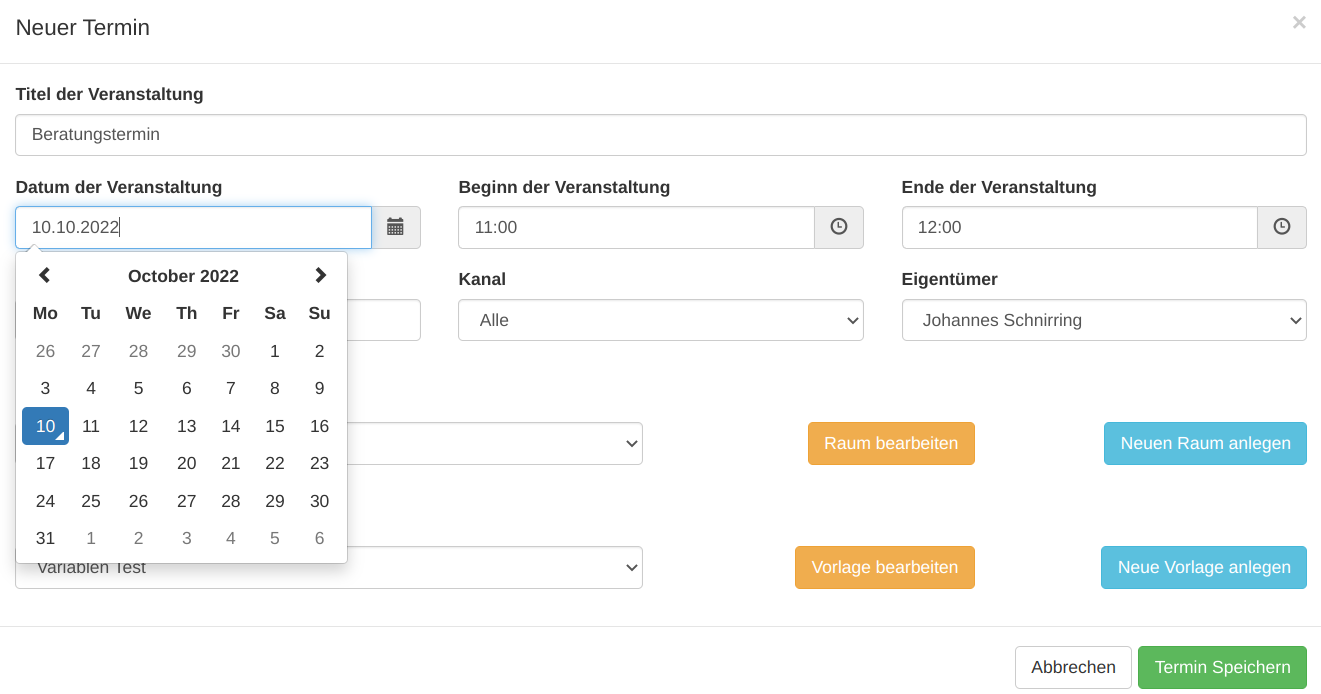
\includegraphics[width=0.9\textwidth]{screen_old_datepicker.png}
\end{figure}

Beim Eintragen mehrere Termine wäre es auch besonders praktisch, dass das zuvor
eingegebene Datum stehen bleibt und direkt ein weiterer Zeitslot für den
gleichen Tag angelegt werden kann, ohne dass er nochmal extra das Datum
auswählen muss. Diem meisten der weiteren Felder sind Dropdown Menüs, mit
wenigen Elemente., Die Auswahl der richtigen Werte kann Oliver Claves schnell
vornehmen. Bei der Auswahl der verknüpften Räume werden beispielsweise die
Räume, die mit seinem Nutzeraccount verknüpft sind, ganz oben in der
Auswahlliste angezeigt. Da eine Beratung in der Regel in den eigen Räumen
stattfindet, ist hier eine schnelle Auswahl für den Normalfall möglich. In
einer Spezialsituation, in der ein größerer Beratungstermin beispielsweise in
einem gemeinsamen Gruppenraum stattfinden, ist aber auch solch eine Auswahl
möglich.

\begin{figure}[h]
    \caption{Dropdown zur Auswahl des Beratungsraums. Der eigene Raum wird immer als oberstes angezeigt}
    \centering
    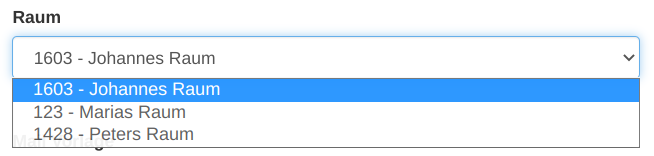
\includegraphics[width=0.9\textwidth]{screen_old_roomdropdown.png}
\end{figure}

Nachdem der Zeitslot für den Termin angelegt ist, wird der entsprechende Tag in
der Kalenderübersicht nun grün hinterlegt. Dies ist ein Zeichen für die
Hilfskräfte der Erstinformation, dass an diesem Tag noch freie Zeitslots
verfügbar sind.

\begin{figure}[h]
    \caption{Kalenderübersicht. Grüne gefärbte Tage zeigen noch freie Zeitslots an. Rot gefärbte Tage weisen auf vergeben Zeitslots hin}
    \centering
    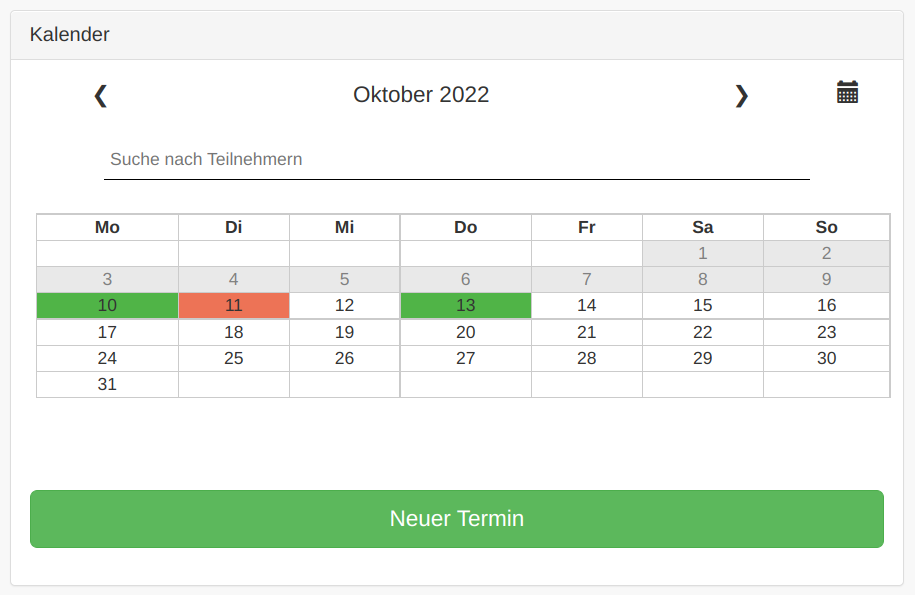
\includegraphics[width=0.9\textwidth]{screen_old_module.png}
\end{figure}

Durch ein Mouseover über den entsprechenden Tag in der Monatsübersicht kann man
die genauen Termine mit Informationen über die Uhrzeit, den zuständigen
Beratenden und die Anzahl der freien Plätze sehen. Oliver Claves erklärt mir,
dass die kompakte Monatsansicht mit den farblich hervorgehobenen Terminslots
bereits eine sehr gute Lösung ist, damit die Hilfskräfte auf einen Blick
erfassen können, an welche Tagen sie den Kunden noch Beratungsgespräche
anbieten können. Sobald alle Plätze der Beratungstermine an einem Tag vergeben
sind, wird dieser im Kalender rot markiert. "So sehen Hilfskräfte sofort, dass
sie hier keinen Termin mehr vergeben werden können", erklärt Herr Claves
\todo{direkte Zitate?}.

\begin{figure}[h]
    \caption{Bewegt man den Mauszeiger über einen Tag, erscheinen weiteren Informationen zu den Zeitslots an diesem Tag}
    \centering
    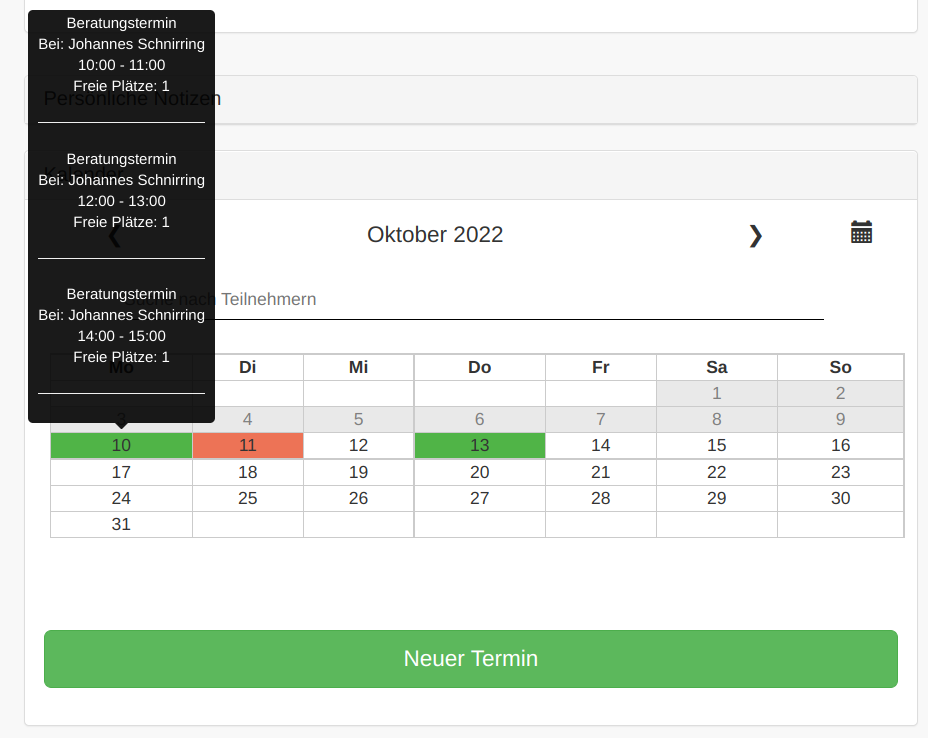
\includegraphics[width=0.9\textwidth]{screen_old_hover.png}
\end{figure}

Soll nun ein Zeitslot tatsächlich vergeben werden, klickt man auf den
entsprechenden Tag in der Monatsansicht und es öffnet sich ein Modal. Dies ist
ein Fenster, welches sich über den anderen Bildschirminhalt legt und dem Nutzer
somit deutlich anzeigt, dass hier eine Aktion im neu geöffnet Fenster notwendig
ist. Oliver Claves zeigt mir, wie die Mitarbeitenden der Erstinformation in
diesem Detail-View die freien Zeitslots an die ratsuchenden Personen vergeben
können. In einer Liste werden, nach Uhrzeit sortiert, alle Termine
untereinander angezeigt. Neben jedem freien Termin steht ein Button zum Vergabe
dieses Zeitslots zur Verfügung.

\begin{figure}[h]
    \caption{Der Detail-View: Eine Liste mit drei freien Zeitslots am entsprechenden Datum}
    \centering
    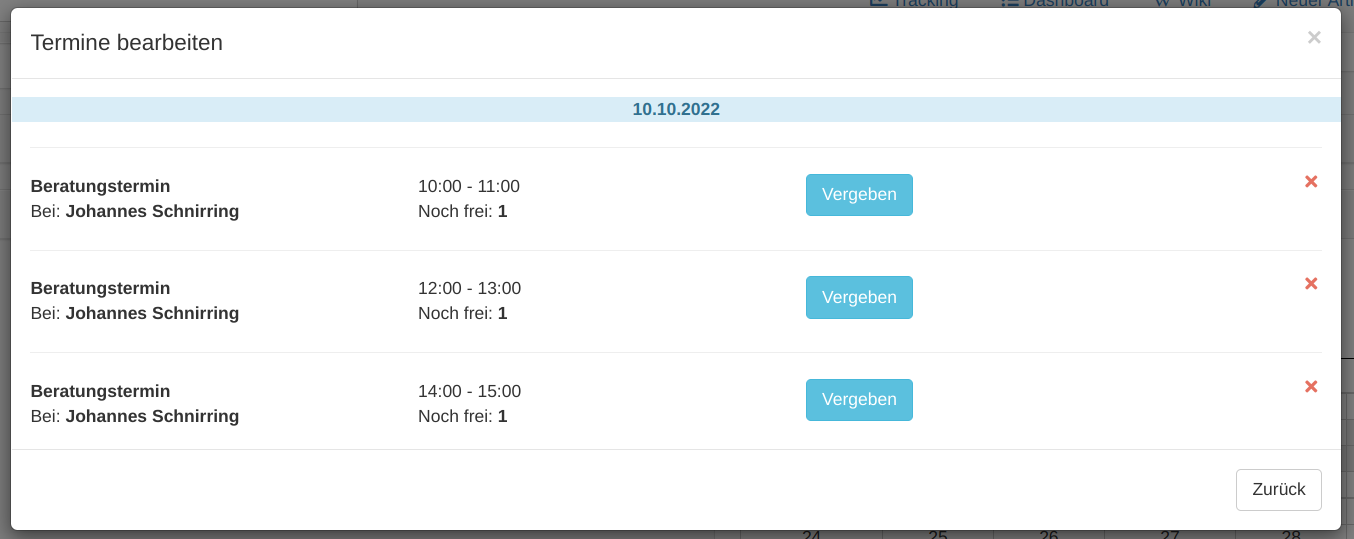
\includegraphics[width=0.9\textwidth]{screen_old_daylist.png}
\end{figure}

Herr Claves zeigt mir wie eine Hilfskraft der Erstinformation nun einen solchen
Zeitslot vergeben könnte. Nach Klick auf den "Vergabe-Button" klappt ein
Formular auf, indem Name, Kontaktdaten und Anliegen der Ratsuchenden erfasst
werden können.

\begin{figure}[h]
    \caption{Formular zum vergeben eines Zeitslots an eine ratsuchende Person}
    \centering
    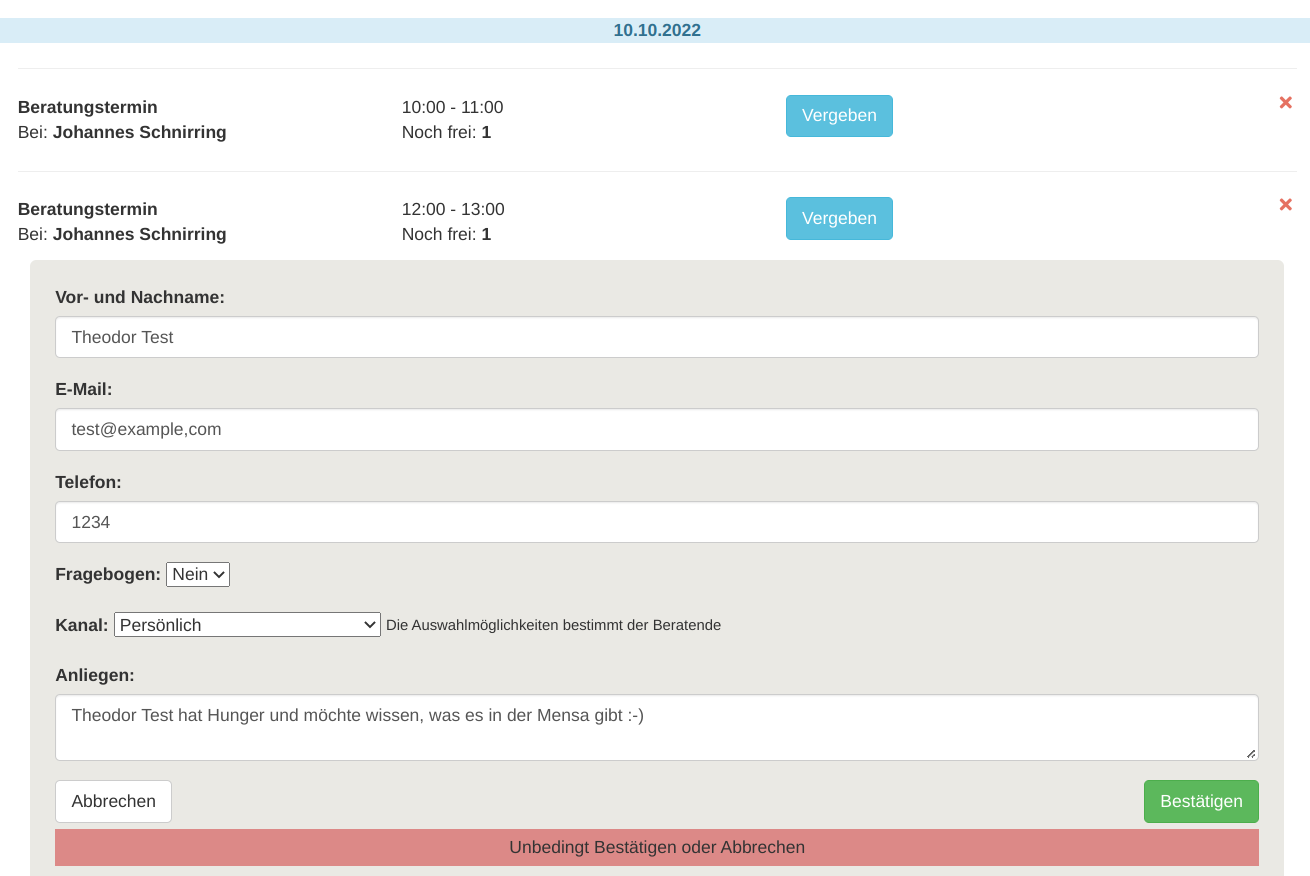
\includegraphics[width=0.9\textwidth]{screen_old_clientdata.png}
\end{figure}

Nachdem alle personenbezogenen Daten korrekt erfasst wurden kann der Termin nun
endgültig gebucht werden. Hierzu klicken die Hilfskräfte auf den Button
"Bestätigen". Oliver Claves erklärt mir, dass dies ein sehr wichtiger Schritt
ist: Solange eine Mitarbeitender der Erstinformation das Formular zum Erfassen
der persönlichen Daten des Ratsuchenden geöffnet hat, wird dieser Zeitslot mit
einer Sperre versehen. So wird verhindert, dass dieser Zeitslot von einem
Kollegen vergeben werden kann, während man selbst gerade mit dem Ratsuchenden
beispielsweise am Telefon die persönlichen Daten und das Anliegen bespricht.
Sollte nach dem Aufklappen des Formulars der entsprechende Zeitslot doch nicht
vergeben werden, ist es deshalb notwendig, dass die terminvergebende Person auf
"Abbrechen" klickt, um die Sperre dieses Zeitslots aufzuheben und ihn somit für
die Kollegen wieder freizugeben. Oliver Claves betont, dass dieser Schritt
manchmal nicht ganz intuitiv ist, und für die Hilfskräfte daher in
Einführungsschulungen immer besonders hervorgehoben wird. Es wäre allerdings
deutlich schlimmer einen Termin doppelt zu vergeben und somit mindestens einer
ratsuchenden Person wieder absagen zu müssen, als einen Zeitslot versehentlich
zu sperren.

\begin{figure}[h]
    \caption{Detail-View: Ein Zeitslot wurde nun vergeben und ist für den entsprechenden Kunden reserviert. Hilfskräfte können nur den Namen des Ratsuchenden einsehen}
    \centering
    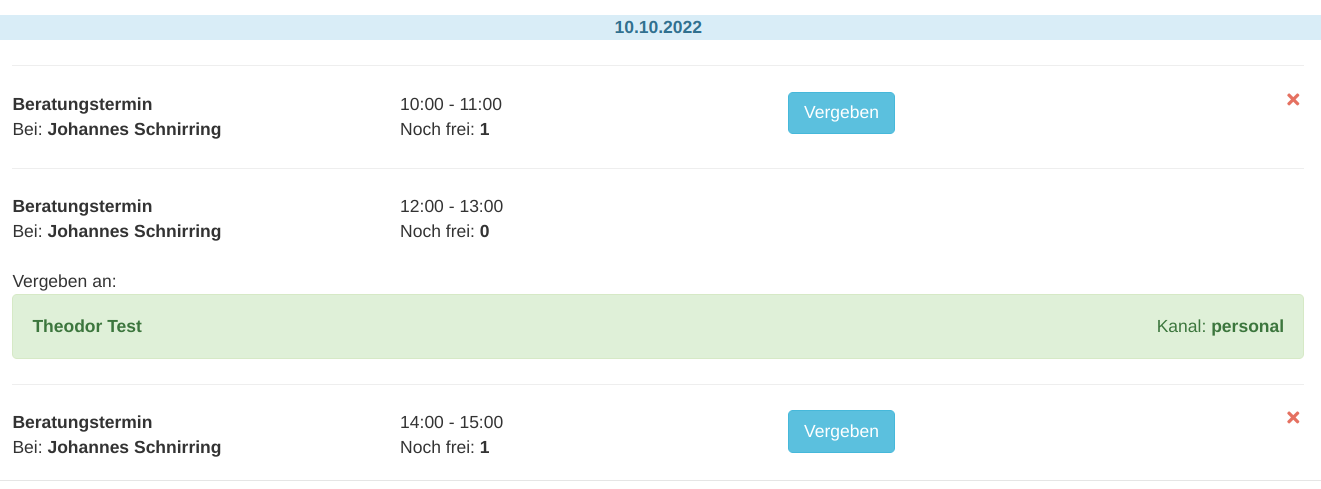
\includegraphics[width=0.9\textwidth]{screen_old_assigned_hiwi.png}
\end{figure}

Ist der Termin nun erfolgreich vergeben, können alle Nutzenden der Software
einsehen an welche Person dieser Termin vergeben wurde. Meldet sich ein
Ratsuchender beispielsweise einige Tage später noch einmal bei der
Erstinformation und möchte wissen, wann sein Beratungstermin stattfindet,
können die Mitarbeitenden der Erstinformation diese Auskunft aus der Software
ablesen. Aus Datenschutzgründen können allerdings keine weiteren
personenbezogenen Daten des Beratungstermins ausgelesen werden. Lediglich der
Studienberatende, bei dem der Termin stattfindet, bekommt beim Aufruf des
Detail-Views weitere Details wie Kontaktdaten und Anliegen der ratsuchenden
Person angezeigt.

\begin{figure}[h]
    \caption{Detail-View: Der verantwortliche Beratende kann weitere personenbezogene Details einsehen}
    \centering
    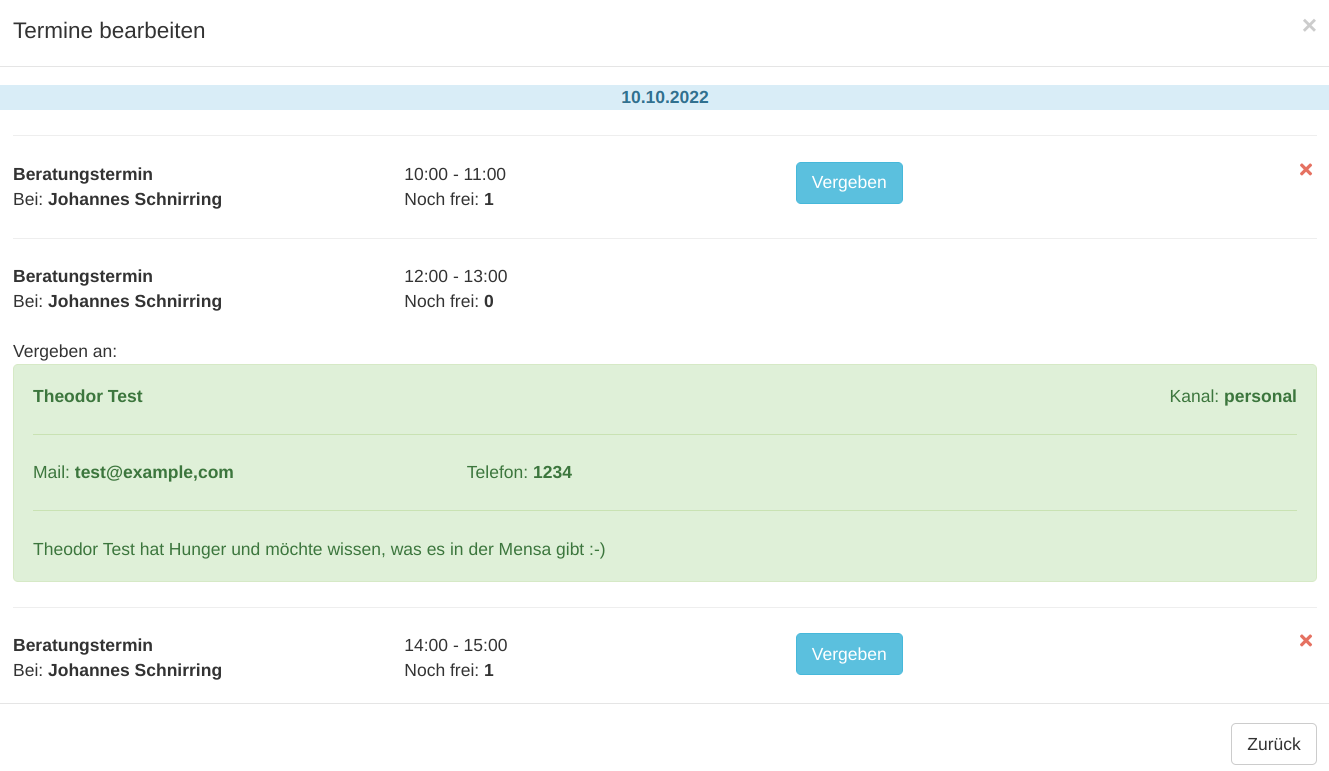
\includegraphics[width=0.9\textwidth]{screen_old_assigned.png}
\end{figure}

Herr Claves hat nun den zweistufigen Workflow zur Terminvergabe einmal komplett
durchgespielt und mich auf viele Details hingewiesen. Während Herr Claves mir
gezeigt und erzählt hat, wie die Terminvergabe in der aktuellen Softwareversion
abläuft, habe ich in Stichworten mitgeschrieben, welche Bemerkungen und
Auffälligkeiten er besonders betont hat.

\subsubsection{Spannende Erkentnisse}
Während bisher der detaillierte Ablauf des Interviews im Kontext geschildert wurde, sollen im Folgenden die wesentlichen Auffälligkeiten nochmals zusammengefasst werden, die während des Interviews notiert wurden. Das Augenmerk liegt hierbei auf Beobachtungen, die Konsequenzen für den Designprozess des überarbeiteten Kalendermoduls zur Terminvergabe hervorbringen.

\begin{itemize}
    \item Datum / Uhrzeit mit Maus statt Tastatur
    \item Suche nach Teilnehmer
    \item Kompakte Ansicht Kalender (mit Farben)
    \item Telefonnummeranzeige ("Silbentrennung")
    \item Format / Beispielwerte bei Variablen in Templates
    \item Modal reset oder nicht?
\end{itemize}

\subsubsection{Erarbeitung von Verbesserungsvorschlägen}

\subsection{Prototyping}
\subsubsection{Methode ???}
\subsubsection{Erste Prototypen}
\subsubsection{Feedback zu Prototypen}

\subsection{Implementierung}
\subsubsection{Methode ???}
\subsubsection{Beschreibung des Prozess}
\subsubsection{Technische Umsetzung}
\subsubsection{Präsentation erster Ergebnisse}

\subsection{Testen / User-feedback}
\subsubsection{Methode ???}
\subsubsection{Feedback der Nutzenden}
\subsubsection{Ausblick auf weitere Iterationen}

\section{Reflektion und Fazit}
\subsection{Beschreibung des Ergebnis}
\subsection{Beurteilung der Umsetzungsphase}
\subsection{Beurteilung der eingesetzten Methoden}
\subsection{Ausblick}

\newpage

\bibliographystyle{plain}
\bibliography{refs}

\end{document}